\documentclass[11pt]{report}
% packages
% Fran Burstall's Bath thesis package
\usepackage{baththesis}
\usepackage{amssymb} %for Blackboard bold etc \usepackage{graphicx} %for including eps graphics % front matter
\usepackage[pdftex]{graphicx} % To include pictures
\usepackage{caption}
\usepackage{subcaption} % To use subfigures with subcaptions
\usepackage{url}
\usepackage{amsmath} % Equations
\usepackage{txfonts}
\setlength{\parskip}{0.9em} %Paragraph spacing
\usepackage{pgfgantt}
\usepackage{cite}
\usepackage{csquotes}
\renewcommand*{\mkcitation}[1]{ #1}

\newcommand{\phim}{\mathbf{\phi}}
\newcommand{\X}{\mathbf{X}}
\newcommand{\x}{\mathbf{x}}
\newcommand{\w}{\mathbf{w}}
\newcommand{\Z}{\mathbf{Z}}
\newcommand{\z}{\mathbf{z}}
\newcommand{\h}{\mathbf{h}}

%\usepackage[hidelinks]{hyperref} % Adds references links without color
\usepackage{hyperref} % Adds references links with color
\usepackage{xcolor}
\hypersetup{
    colorlinks,
    linkcolor={red!50!black},
    citecolor={blue!50!black},
    urlcolor={blue!80!black}
}

\title{Visual Effects} \author{Ieva Kazlauskaite, Garoe Dorta-Perez, Richard Shaw}
%\degree{Doctor of Philosophy}
\unit{ unit }
\department{Department of Computer Sciences} \degreemonthyear{May 2015}
\norestrictions

\begin{document}
\maketitle

\chapter{Introduction}
\label{ch:intro}
\begin{center}
\textquote[~\cite{Attenborough:1998}]{\textit{Birds are the most accomplished aeronauts the world has ever seen. They fly high and low, at great speed, and very slowly. And always with extraordinary precision and control}.}
\end{center}


\chapter{Previous Work}
\label{sec:previous}

\section{Data Capture}


\section{Sparse Reconstruction}


\section{Blendshape Optimisation}


\section{Skin Rendering}

Rendering realistic skin is a challenging task.
As social beings, we interact with each other on a daily basis, humans perception is quite sensitive to skin appearance, specially with faces.
Skin is composed of several layers with different properties, to accurately simulate skin, the light transport between this layers has to be modelled.
The full effect of light scattering between two points on the surface can be modelled using a Bidirectional Surface-Scattering Distribution Function (BSSRDF).

\cite{Weyrich2006} two layer model captured with light dome. 
\cite{Donner2008} layered model for haemoglobin in skin.
\cite{Jimenez2010} haemoglobin for different blendshapes.

Normal maps are use to alter the normals of the scene objects during rendering.
This technique is used to add geometric detail to an object at rendering time without actually changing the geometry.
The error introduced with this approach is shown in Figure \ref{fig:normal_map}, a ray $r_1$ hist the geometry at point $p$ and the normal $n_p$ is used for shading, while if we had the based geometry the hitting point would be $p'$ and the normal $n'$.
Normal maps are for skin rendering are usually captured using expensive light domes with a number of synchronized cameras. 

\cite{Tian2011} Survey on super-resolution imaging.
\cite{Jianchao2010} Super resolution with dictionary learning.
\cite{Hertzmann2001} Image analogies paper.
\cite{Graham2013} microgeometry and Image Analogies, the one we are implementing.

\begin{figure}[htbp!]
\centering
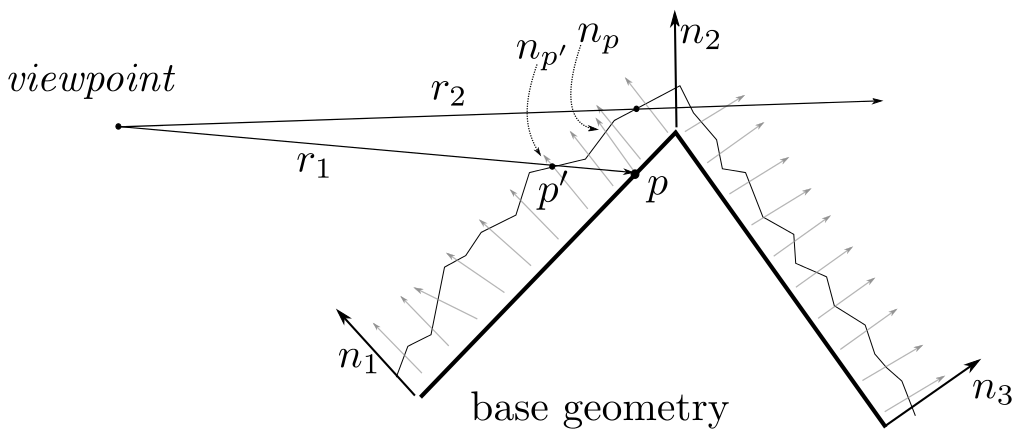
\includegraphics[width=0.7\textwidth]{img/normal_map}
	\caption{ Using normal maps to simplify a given geometry, image taken from \cite{ganovelli2014}.}
	\label{fig:normal_map}
\end{figure}



%-----------------------------------------------------------------------
\chapter{Methodology}
\label{sec:methods}


\section{Data Capture}


\section{Sparse Reconstruction}


\section{Blendshape Optimisation}


\section{Skin Rendering}

\cite{Hertzmann2001} Image analogies paper.


%-----------------------------------------------------------------------
\chapter{Results}


%-----------------------------------------------------------------------
\chapter{Conclusions}

\bibliographystyle{eg-alpha}
\bibliography{baththesis}

\end{document}